% REVISÃO DE LITERATURA--------------------------------------------------------

\chapter{REVISÃO DE LITERATURA}
\label{chap:fundamentacaoTeorica}

A base teórica necessária para a realização da pesquisa e o entendimento do estudo é apresentada nesse capítulo, destacando os conceitos de exoma, Sequenciamento do DNA, \textit{Copy Number Variation}, \textit{Change Point Detection}, algoritmos relacionados a CPD, como o \textit{Circular Binary Segmentation}, \textit{Graph Spectrum}, PELT, entre outros. Além desses tópicos o trabalho apresenta a descrição de Matriz de Confusão, e as suas fórmulas, para a determinação da eficiência de algoritmos. Esses conceitos apresentados possuem a finalidade de reunir evidências e contribuições sobre o uso do processo de algoritmos de detecção de pontos de mudança no contexto de anotação de \textit{copy number variation}.

\section{EXOMA}
\label{sec:exoma}

O genoma é constituído de regiões codificantes e não codificantes, elas são denominadas como \textit{éxons} e \textit{íntrons} respectivamente. A região codificante constituí-se de sequências de proteínas, elas representam cerca de 1\% do genoma \cite{Ng2009}. A \autoref{fig:figura-exoma} é uma representação de possíveis regiões presentes na estrutura do DNA e RNA, sendo que as áreas destacadas com uma camada colorida são classificadas como \textit{éxons} e em cada espaço existente entre essas camadas são categorizados como \textit{íntrons}.

\begin{figure}[!htb]
    \centering
    \caption{Exemplificação das regiões codificantes de proteínas (\textit{éxons} ou exoma) na estrutura do DNA e RNA}
    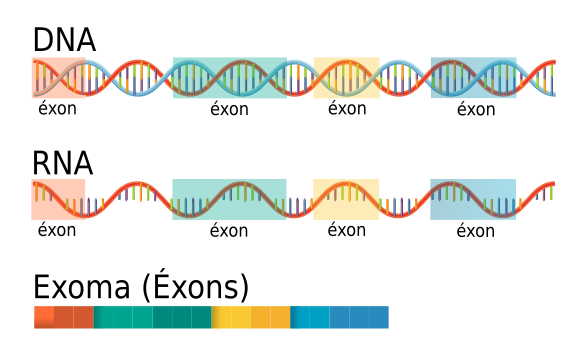
\includegraphics[width=0.8\textwidth]{./dados/figuras/exoma}
    \fonte{Autoria Própria}
    \label{fig:figura-exoma}
\end{figure}

A quantidade de 1\% do genoma pode chegar a conter cerca de 180 mil \textit{éxons}, esse conjunto de regiões codificantes de proteínas é conhecido como exoma, como representado na \autoref{fig:figura-exoma}, essa representação é formada ao unir todos os éxons existente no DNA \cite{Bamshad2011}. O exoma pode ser obtido pelo processo de sequenciamento completo do exoma (WES), que é correspondente a separação dos \textit{éxons} contidos no genoma, por uma série de etapas. O seu uso vem sendo registrado como base para realizar demasiados diagnósticos moleculares de detecção de distúrbios genéticos, por ser possível identificar variantes relacionadas a doenças com as informações geradas \cite{Bamshad2011,Lee2014,HutchisonIII2007}.

Apesar da aplicação do sequenciamento para obtenção do exoma através da extração dos \textit{éxons}, ainda existem dúvidas sobre quais regiões são exatamente codificantes de proteínas, assim não podendo ser especificado qual o exato conjunto equivalente ao exoma \cite{Bamshad2011}.

A utilização do teste de sequenciamento do exoma possibilitou um rendimento de 25–35\% em diagnósticos de doenças raras de origem genética \cite{Bamshad2011}. Entretanto, a utilização das informações produzidas não se contém a somente análise de distúrbios. Grandes esforços por parte de pesquisadores biomédicos, empresas de biotecnologia e medicamentos, agências financiadoras e grupos de pacientes, estão sendo direcionados na descoberta das funcionalidades, relações e reações que cada gene possui de acordo com alguma variação ao qual o mesmo foi disposto \cite{Antonarakis2006}.

% Associar o exoma ao CNV 
O WES vem sendo utilizado em demasiados cenários oriundos de variações gênicas, como em descobertas de perda auditiva \cite{Likar2018}, encefalopatia epiléptica \cite{Allen2016}, mutação gerada a partir de uma determinada doença \cite{Lin2019}, hipotireoidismo congênito \cite{Fu2019}, entre outros. Essas pesquisas são realizadas utilizando conjuntos de amostras de indivíduos com características semelhantes ou extremamente opostas \cite{Bamshad2011}, para que sejam analisadas e comparadas, na tentativa de identificar onde alguma variação no número de cópias está situada e se ela causa algum comportamento inesperado.

\section{SEQUENCIAMENTO DO DNA} 
\label{sec:sequenciamentoDoDna}

% Sobre o sequenciamento
O estudo acerca do DNA e das informações contidas nele obteve um grande impulso por parte de vários cientistas do mundo inteiro no século XX, e com isso surgiu um movimento responsável pela investigação dos componentes do DNA, denominado como o Projeto Genoma Humano \cite{Lander2001}. Esse projeto levantou investimentos científico e capital, com um orçamento variando entre US\$3 bilhões a US\$53 bilhões, para obter mais entendimento das características do DNA a partir do sequenciamento completo do genoma (WGS) \cite{Marian2011}.

% Objetivo de sequenciamento 
Com o objetivo de ordenar os nucleotídeos do DNA, decodificando o código genético \cite{Edwards2011}, as primeiras pesquisas relacionadas ao sequenciamento surgiu próximo ao final do século XX, com variadas propostas acerca do assunto. Uma das propostas era criação de tecnologias capazes de identificar a sequência completa do genoma humano, mapeando cada partícula existente \cite{Lander2001,HutchisonIII2007}.

A tarefa de sequenciar o genoma humano completo no projeto consumou alguns anos para ser finalizada, sendo iniciada em 1990 e concluída oficialmente em 2003, apesar de conter mais de 5000 cientistas em centros de pesquisas dos Estados Unidos, Europa e Japão, envolvidos nessa tarefa \cite{HutchisonIII2007}. A sua conclusão tardia se deu por possuir uma certa complexidade ao montar e ordenar os pequenos pedaços sequenciados corretamente, além de demandar um enorme custo estimado em 3 bilhões de dólares para a análise do conjunto de cadeias do DNA \cite{Rye2017,HutchisonIII2007}.

% Primeiro sequenciamento 
As tecnologias desenvolvidas para o sequenciamento tende a se desenvolver incrementalmente, utilizando algumas particularidades dos métodos existentes e melhorando-os conforme a necessidade da realidade atual \cite{HutchisonIII2007}. Entre os métodos pesquisados e desenvolvidos ao longo dos anos, o que mais se destacou e foi utilizado no Projeto do Genoma Humano foi o método de Sanger, desenvolvido por volta de 1970 \cite{Sanger1975} e usado no WGS \cite{HutchisonIII2007}. O sucesso desse método se deu pela disponibilização de um alto nível de qualidade ao ler uma sequência curta do DNA \cite{Edwards2011}. Ele possibilitou a análise dos segmentos do genoma vistos microscopicamente, como os cromossomos e as variações contidas em sua estrutura, usadas para visualizar as diferenças entre outras amostras de genomas estudados \cite{Feuk2006,Sanger1975}.

% Desvantagem e evolução do método/Explicar os modelos de sequenciamento https://www-nature.ez48.periodicos.capes.gov.br/articles/nrg2626#df3 
Apesar de o sequenciamento de Sanger suprir as expectativas em sua época de sua criação e ainda ser utilizado em vários casos da atualidade, ele apresentava um custo elevado ao sequenciar genomas complexos, sendo estimado em 1 dólar por base de DNA sequenciada, o que dava em média 3 bilhões de dólares por genoma completo na época do projeto \cite{HutchisonIII2007}. Esse fator ajudou a motivar o estudo de novos procedimentos capazes de obter aumento no desempenho e custos mais acessíveis em comparação com os existentes.

A partir dessa realidade surgiu vários métodos baseados no \textit{next-genaration sequencing} (NGS), esses métodos são um conjunto de planos executados em conjunto para obter uma coleção maior de dados com um custo reduzido e melhor desempenho \cite{Metzker2010,Zhao2013}, como visto nos resultados produzidos pelos sequenciadores do Solexa \cite{Bennett2004}, HiSeq 2000, SOLID e outros \cite{Edwards2011,Linnarsson2010}. Esses equipamentos estão possibilitando uma maior cobertura e resolução, assim sendo possível identificar mais variações no número de cópias do genoma sequenciado \cite{Zhao2013}.

% Explicação técnica de como sequencia? 

% Introdução a análise computacional 
O início da análise computacional dos dados de sequenciamento foi abordado por Duncan McCallum e Michael Smith \cite{McCallum1977}, ao desenvolver um dos primeiros programas direcionados a compilação e estudo das informações sequenciadas \cite{HutchisonIII2007}. Entretanto, a criação de programas computacionais não se deteve com a evolução das técnicas de sequenciamento, assim sendo estudado e desenvolvidos novas formas de observações automatizadas para acompanhar a trajetória evolutiva das ferramentas de sequenciamento do DNA.

% Explicar os dados gerados Dataset e como estão disponíveis 

\section{COPY NUMBER VARIATION} 
\label{sec:copyNumberVariation}

% Introdução ao assunto do CNV 
A \textit{copy number variation} (CNV) ou no português, variação no número de cópias, são alterações que ocorrem na região genômica, elas se classificam como inserções, duplicações e deleções na estrutura do cromossomo, como representado na \autoref{fig:figura-copy-number-variation} \cite{Zhao2013,Redon2006}. Essas variações podem ser encontradas em todos os seres humanos, podendo não representar nenhuma alteração ou ser responsável por doenças de origem mendeliana, sua existência e descoberta são essenciais para o entendimento da composição genômica \cite{Redon2006,Feuk2006}.

% Definição de CNV com imagem
\begin{figure}[!htb]
    \centering
    \caption{Exemplo de variações no número de cópias (CNVs) no cromossomo}
    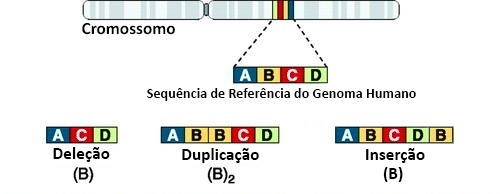
\includegraphics[width=1\textwidth]{./dados/figuras/copy-number-variation}
    \fonte{Adaptado de \cite{Dierssen2009}}
    \label{fig:figura-copy-number-variation}
\end{figure}

% Contexto 
Com o estudo do genoma humano \cite{Lander2001} houve a possibilidade de descobertas relevantes sobre doenças ao comparar a composição do DNA de várias pessoas, entretanto, inicialmente essas descobertas se deu no nível macro, como em números de cromossomos. Portanto, a maior parte das doenças encontradas estavam relacionadas a análise do genoma completo, onde podiam ser vistos a partir de um microscópio \cite{Feuk2006}.

As tecnologias de sequenciamento do DNA possibilitou a investigação das micropartículas que concebiam o genoma, a partir dela foi possível identificar a existência de pequenas inserções, deleções e duplicações não identificadas a partir de análises microscópicas. De acordo com o estudo dessas variações no número de cópias da estrutura genômica, foram vistos uma série de casos onde não representava nenhuma consequência e outros que possuíam uma grande chance de causar doenças de origem mendelianas \cite{Feuk2006,Xi2011}.

% Sobre o estudo 
O estudo do CNV foi pouco aprofundado até recentemente em comparação com outras classes da variação genética \cite{Redon2006}, mas com o avanço do NGS e o auto rendimento produzido pelos sequenciamentos utilizados, houve um aumento no grau de avaliabilidade dos mesmos, sendo possível o reconhecimento das regiões afetadas pelas CNVs, assim mudando essa realidade \cite{Mills2011,Feuk2006}.

As distribuições de variações do número de cópias se distinguem entre populações, elas são formadas por mutação, seleção e histórico demográfico, onde indivíduos que se encontram expostos a determinadas características como, por exemplo, demográfica, apresentam variações semelhantes, assim sendo possível a identificação e classificação entre categorias de populações existentes \cite{Redon2006}.

Em \cite{Snijders2001} é feita uma montagem de dados genômicos, de modo a mostrar as variações existentes e as medições precisas da amostra sequenciada pelo \textit{Coriell Institute for Medical Research}. Os dados dessa amostra, serão denominados como Coriell neste trabalho pela ligação com o instituto pesquisado, ela é utilizada em pesquisas por oferecer medições confiáveis das variações ocorridas.

As alterações nos números de cópias apresentadas em Coriell, atende a várias origens, inclusive as variações recorrentes a câncer. As informações sequenciadas são dispostas em microarrays, elas podem ser montadas graficamente sendo formando uma relação de razão logarítmica média $_2$ (razão de $log_{2}$) pela posição ou pelo cromossomo, como apresentado na \autoref{fig:coriell-cnv}.

\begin{figure}[!htb]
    \centering
    \caption{Dados genômicos da amostra de DNA pertencente ao Coriell, referente a linhagem celular GM03576}
    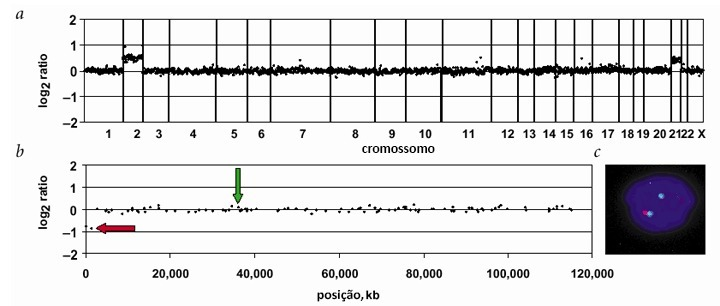
\includegraphics[width=1\textwidth]{./dados/figuras/coriell-cnv}
    \fonte{Adaptado de \cite{Snijders2001}}
    \label{fig:coriell-cnv}
\end{figure}

A linhagem celular GM03576, pertencente ao conjunto de dados do Coriell, demonstra a identificação de CNVs de acordo com a representação gráfica. A \autoref{fig:coriell-cnv}-a denota o ganho de números de cópias do cromossomo 2 e 21, onde é possível ver um aumento na média da razão de $log_{2}$. A \autoref{fig:coriell-cnv}-b destaca a deleção de números de cópias de acordo com o cromossomo 9 da linhagem celular apresentada, onde contém setas de identificação.

O \cite{Snijders2001}, apresenta uma confirmação dos ganhos e perdas relatados acima, na \autoref{fig:coriell-cnv}-c, destacando os ganhos como pontos na cor verde e a perda como pontos na cor vermelha.

\subsection{Métodos de Detecção} 

De modo a estudar e descobrir as principais características acerca das regiões do genoma, sendo elas a codificante e a não codificante, a investigação da detecção das variações no número de cópias é essencial para o processo de descoberta de peculiaridades relacionadas a amostras. Para alcançar esse objetivo, \cite{Zhao2013} descreve existe cinco estratégias diferentes a serem aplicadas na detecção, sendo elas as detalhadas na \autoref{fig:estrategias-deteccao-cnv}.

\begin{figure}[!htb]
    \centering
    \caption{Estratégias de detecção de variações no número de cópias}
    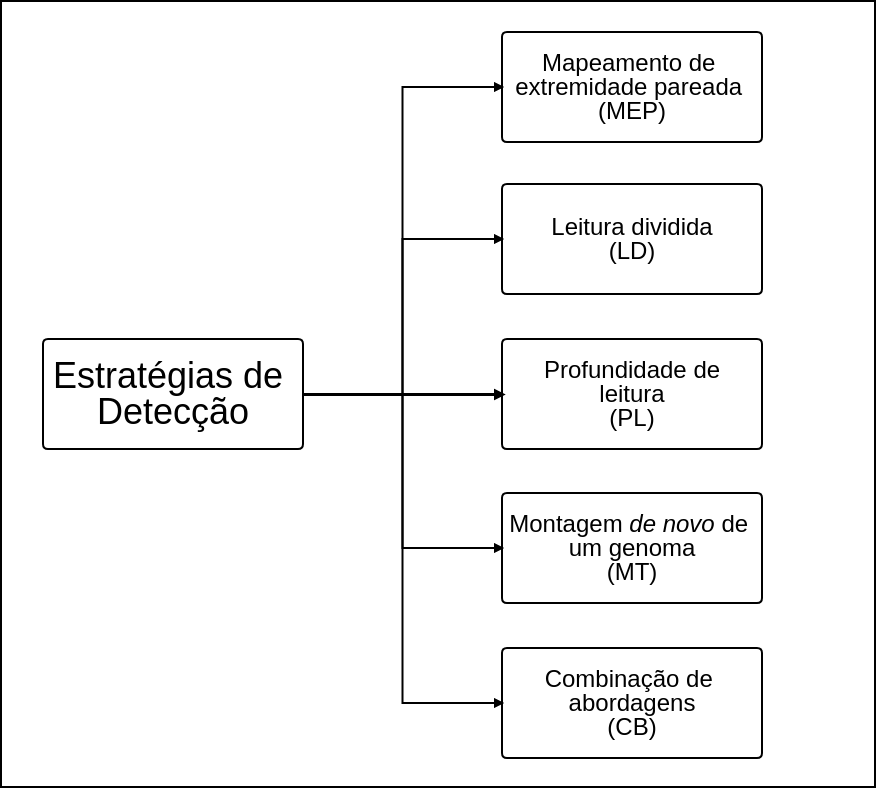
\includegraphics[width=0.8\textwidth]{./dados/figuras/estrategias-deteccao-cnv}
    \fonte{Autoria Própria}
    \label{fig:estrategias-deteccao-cnv}
\end{figure}

As abordagens da \autoref{fig:estrategias-deteccao-cnv} apresenta vantagens e limitações de acordo com o cenário a ser aplicado. Varias vantagens foram registradas, como no MEP em utilizações em leituras de final emparelhadas, ou em ferramentas que utilizam a abordagem LD, onde apresenta mais desempenho em leituras curtas, mas independente disso, nenhuma das cinco abordagens conseguiram detectar todas as CNVs existentes \cite{Zhao2013}.

O desenvolvimento de aplicações ligadas a essas estratégias se dá em linguagens de programação como R, C/C++, Java e outras. Apresentando diferentes abordagens para que a \textit{copy number variation} seja identificada e exposta, tentando alcançar uma maior desempenho \cite{Zhao2013}.

\subsection{Métodos Avaliados} 

Nesta subseção será apresentado a descrição alguns métodos focados na análise de \textit{copy number variation} que utilizam a estratégia de detecção baseada em profundidade em leitura (PL), ou seja, aplicações que implementam modelos estatísticos focados em encontrar pontos de mudanças em uma série temporal, para alcançar o objetivo de encontrar a variação em dados do cromossomo \cite{Zhao2013}. A maioria das ferramentas descritas a seguir possuem natureza \textit{opensource} (Código livre), assim sendo possível obter e contribuir com o código para o seu crescimento, com essa característica em mente, a evolução do mesmo pode ocorrer apos a publicação deste estudo, alterando a versão listada na \autoref{qua:ferramentas-de-deteccao-de-cnv}.

% Detecção
A detecção de CNVs passou por tecnologias como cariotipagem e hibridização fluorescente in situ (FISH) no início de pesquisas relacionadas ao tema, apos a descoberta da estrutura genômica completa, a detecção se deu através de hibridização genômica comparativa baseada em array (aCGH). O NGS possibilitou a melhoria na leitura de variações no número de cópias, obtendo uma maior desempenho ao ler os identificar as regiões variantes graças as novas técnicas de sequenciamento \cite{Zhao2013}. 

O método de identificação de CNV aplicado a dados gerados com ferramentas do NGS baseado em PL é utilizado para estimar o número de cópias, determinando sua localidade de acordo com as posições existente do cromossomo de amostra. A descoberta de CNVs segue quatro passos ao utilizar essa abordagem: mapeamento, normalização, estimativa do número de cópias e segmentação \cite{Zhao2013}.

A estimação do número de cópias pode ser resolvida de forma a aplicar algoritmos nos dados da amostra, como pode ser visto em algumas ferramentas existentes de detecção de CNVs presentes no \autoref{qua:ferramentas-de-deteccao-de-cnv}. Esses modelos assumem a existência de perdas ou ganhos ao longo do cromossomo, aplicando algoritmos de distribuição de probabilidade na média e/ou variância, de modo a detectar a localização de alguma variação no número de cópias \cite{Zhao2013}.

% ##### define colors
\definecolor{color000000}{RGB}{0,0,0}
% ##### FIM define colors

% ######## init table ########
\begin{table}[h]
 \centering
% distancia entre a linha e o texto
 {\renewcommand\arraystretch{1.25}
 \caption{Ferramentas de detecção de CNVs usando a abordagem de profundidade em leitura\label{qua:ferramentas-de-deteccao-de-cnv}}
 \begin{adjustbox}{max width=\textwidth}
\begin{tabular}{ l l l l l }
  \cline{1-1}\cline{2-2}\cline{3-3}\cline{4-4}\cline{5-5}  
    \multicolumn{1}{|c|}{\textbf{\textcolor{color000000}{Ferramenta}}} &
    \multicolumn{1}{c|}{\textbf{\textcolor{color000000}{Versão}}} &
    \multicolumn{1}{c|}{\textbf{\textcolor{color000000}{Linguagem}}} &
    \multicolumn{1}{c|}{\textbf{\textcolor{color000000}{Método}}} &
    \multicolumn{1}{c|}{\textbf{Referência}}
  \\  
  \cline{1-1}\cline{2-2}\cline{3-3}\cline{4-4}\cline{5-5}  
    \multicolumn{1}{|c|}{DNAcopy} &
    \multicolumn{1}{c|}{1.58.0} &
    \multicolumn{1}{c|}{R} &
    \multicolumn{1}{c|}{Segmentação binária circular (CBS)} &
    \multicolumn{1}{c|}{\cite{Olshen2004}}
  \\  
  \cline{1-1}\cline{2-2}\cline{3-3}\cline{4-4}\cline{5-5}  
    \multicolumn{1}{|c|}{fastseg} &
    \multicolumn{1}{c|}{1.30.0} &
    \multicolumn{1}{c|}{R} &
    \multicolumn{1}{c|}{Estrutura Bayesiana} &
    \multicolumn{1}{c|}{\cite{Baldi2001}}
  \\  
  \cline{1-1}\cline{2-2}\cline{3-3}\cline{4-4}\cline{5-5}  
    \multicolumn{1}{|c|}{iSeg} &
    \multicolumn{1}{c|}{1.3.2} &
    \multicolumn{1}{c|}{C++} &
    \multicolumn{1}{c|}{\textit{T-}testes simples para calcular \textit{p-}valores} &
    \multicolumn{1}{c|}{\cite{Girimurugan2018}}
  \\  
  \cline{1-1}\cline{2-2}\cline{3-3}\cline{4-4}\cline{5-5}  
    \multicolumn{1}{|c|}{CGHSeg} &
    \multicolumn{1}{c|}{1.0.2} &
    \multicolumn{1}{c|}{R} &
    \multicolumn{1}{c|}{Modelos lineares misto} &
    \multicolumn{1}{c|}{\cite{Picard2011}}
  \\
  \cline{1-1}\cline{2-2}\cline{3-3}\cline{4-4}\cline{5-5}  
    \multicolumn{1}{|c|}{ExomeDepth} &
    \multicolumn{1}{c|}{1.1.10} &
    \multicolumn{1}{c|}{R} &
    \multicolumn{1}{c|}{Modelo beta-binomial para ajuste de profundidade} &
    \multicolumn{1}{c|}{\cite{Plagnol2012}}
  \\ 
  \hline

 \end{tabular}
 \end{adjustbox}}
\end{table}

Os projetos apresentados no \autoref{qua:ferramentas-de-deteccao-de-cnv} possui suas peculiaridades de acordo com o método utilizado para identificação de CNVs, sendo alguns deles adaptados especificamente para a sua análise, como nos algoritmos implementados no DNAcopy, fastseg, CGHSeg, ExomeDepth. O iSeg é o único listado que se difere das ferramentas citadas acima, oferecendo uma análise genômica que abrange variação do número de cópias do DNA, ocupação do nucleossomo, sensibilidade à nuclease e dados de sensibilidade diferencial à nuclease \cite{Girimurugan2018}.

\section{CHANGE POINT DETECTION}
\label{sec:changePointDetection}

% Introdução ao assunto CPD 
O estudo de dados coletados e distribuídos ao longo de um determinado tempo, também denominado como série temporal (\textit{Time Serie}/TS), é uma área muito utilizada para a observação, previsão e aprendizado de padrões em diversos ramos da ciência. Um problema recorrente ao analisar TS é a identificação de um ponto de variação que não era esperado no decorrer dos dados transcritos no gráfico, essa atividade é denominado como \textit{Change Point Detection} (Detecção de Ponto de Mudança/CPD) \cite{Aminikhanghahi2017}.

\begin{figure}[!htb]
    \centering
    \caption{Exemplo de série temporal com pontos de mudança}
    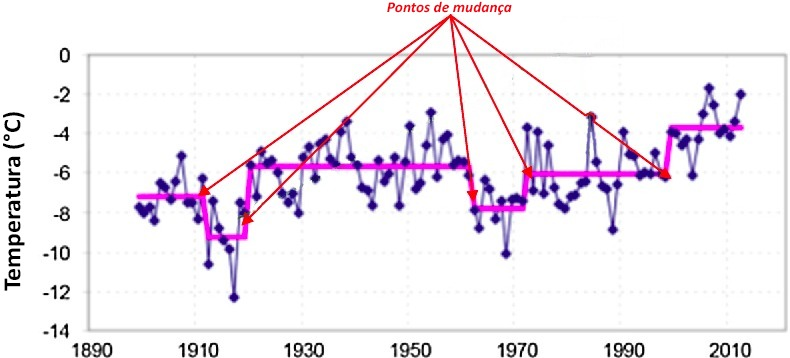
\includegraphics[width=0.8\textwidth]{./dados/figuras/pontos-de-mudanca}
    \fonte{Adaptado de \cite{Aminikhanghahi2017}}
    \label{fig:change-point}
\end{figure}

% Imagem e explicação de CPD de acordo com ela 
Ao observar a \autoref{fig:change-point}, é possível perceber que os elementos da série não permanecem em um único formato, variando em alguns pontos quando há alguma interferência no comportamento do componente percebido. A identificação das setas em vermelho exibe os pontos de mudança e as linhas horizontais na cor rosa são caracterizadas pelos estados normais da série temporal. A observação de pontos de mudanças em uma coleção de dados (\textit{dataset}) com muitos variantes, muitas vezes necessita da utilização de algoritmos, de modo a obter uma maior precisão em sua detecção.

A aplicação desse conceito tem sido bastante explorada em vários cenários na atualidade, como em análises de imagem, reconhecimento de padrões, biomédico \cite{Fan2015}, \textit{cybersecurity} \cite{Polunchenko2012}, séries climáticas \cite{Bates2012}, entre outros. Os objetivos fixados ao estudar pontos de mudança geralmente estão entre saber se existe alguma variação, e se existir identificar se é mais de uma e quais os seus respectivos locais em um determinado tempo \cite{Chen1-2000}.

\subsection{Formulação do Problema}

Seja $X_1, X_2, ..., X_n$ uma sequência de vetores aleatórios independentes (variáveis) com funções de distribuição de probabilidade $F_1, F_2, ..., F_n$, respectivamente. Então, o problema de \textit{change point} é testar a seguinte hipótese nula:

\begin{equation}
    H_0 : F_1 = F_2 = ... = F_n
    \label{eq:cpd-hupotese-nula-1}
\end{equation}

versus a hipótese alternativa

\begin{equation}
    H_{1} : F_{1} = ... = F_{k_1}\neq F_{{k_1}+1} = ... = F_{k_2}\neq F_{{k_2}+1} = ... F_{k_q}\neq F_{{k_q}+1} ... = F_{n},
    \label{eq:cpd-hipotese-alternativa-1}
\end{equation}

onde $1 < k_1 < k_2 < ... < k_q <n$, $q$ é o número desconhecido de pontos de mudança e $k_1, k_2, ..., k_q$ são as respectivas posições que devem ser estimadas. Se as distribuições $F_1, F_2, ..., F_n$ pertencem a uma família paramétrica comum $F(\theta)$, 
então o problema do ponto de mudança é testar hipóteses sobre os parâmetros da população $\theta_i$, com a sequência $i = 1 ..... n$

\begin{equation}
    H_0 : \theta_{1} = \theta_{2} = ... = \theta_{n} = \theta (desconhecido)
    \label{eq:cpd-hupotese-nula-2}
\end{equation}

versus a alternativa

\begin{equation}
    H_1 : \theta_{1} = ... = \theta_{k_1} \not = \theta_{{k_1}+1} = ... = \theta_{2} \not = ... \not = \theta_{{k_q}-1} = ... = \theta_{k_q} \not = \theta_{{k_q}+1}... = \theta_{n},
    \label{eq:cpd-hipotese-alternativa-2}
\end{equation}

onde $q$ e $k_1, k_2, ..., k_q$ precisam ser estimados. Essas hipóteses combinadas revelam aspectos da inferência de ponto de mudança, ou seja, os objetivos citados acima.

As hipóteses apresentadas se adéquam a problemas relacionados a busca de um simples ponto de mudança, entretanto, ela pode ser adaptada para aderirem problemas de múltiplos pontos de mudança em uma coleção de dados \cite{Chen1-2000}.

\subsection{Tipos de Pontos de Mudança}

Os pontos de mudança podem ser observados a partir de uma representação gráfica das distribuições dos valores de uma coleção. Contudo, as mudanças ocorridas podem ser classificadas de acordo com a forma da mudança, seja ela, mudança na média, na variância, em ambos simultaneamente, além de várias categorias de modelos propostos ao longo do tempo \cite{Chen2-2000}.

A aplicação desses modelos de ponto de mudança é apresentada por diversos autores, assim como em \cite{Cheon2010} ao apresentar uma utilização da detecção por média em um modelo Bayesian e em \cite{Shi2017} ao descrever a utilização de um modelo baseado em grafos para análise de modelos de grande dimensão.


% A detecção de pontos de mudança pode ser classificada de duas formas, Online e Offline, onde a forma online é um processamento de dados ao vivo, tentando detectar o ponto antes que ocorra realmente. O método de detecção offline possui uma maior flexibilidade em relação ao online, sendo capaz de analisar toda a série disponível para realizar as identificadões necessárias \cite{Aminikhanghahi2017}.
% Abordar as formas que são utilizadas para identificar


% Ligar CPD ao CNV
% A CPD é explorada em diversos campos de estudo por ser um tópico relevante no observação de uma coleção, com o surgimento do NGS houve um grande aumento em pesquisas relacionadas a análise de ponto de mudança focados em CNV, impulsionando o desenvolvimento de aplicações que usam os algoritmos propostos na formulação de \textit{Change Point Detection} \cite{Xi2011}.

\subsection{Algoritmos Relacionados}

Nesta subseção será apresentado algoritmos desenvolvidos com o proposito de segmentar \textit{datasets} e determinar pontos de mudanças caso haja. Os algoritmos apresentados possuem características de determinação de \textit{change point} divergentes, ou seja, cada um deles possuem uma abordagem própria para a segmentação dos dados \cite{Aminikhanghahi2017}. A seguir encontra-se a definição de algumas ferramentas disponíveis para utilização e contribuição, distribuídas de forma (\textit{open source}):

\subsubsection{CBS}

O CBS (\textit{Circular Binary Segmentation}) é uma modificação de uma estratégia de segmentação binária, proposta com a finalidade de segmentar o cromossomo, apresentando funcionalidades adicionais para normalizar os dados. A segmentação binária é uma técnica aplicada para a determinar a localização de um ponto de mudanças com a aplicação de testes recursivos \cite{Olshen2004}.

Um dos objetivos na proposta do CBS foi a identificação de segmentos menores dentro de segmentos maiores de mudanças. Devido a níveis de significância pequenos aplicados aos cálculos uma grande quantidade de permutações é realizada na determinação de somente um ponto de mudança, chegando a ordem de dez mil, esse processo é feito para cada segmento existente na coleção de dados \cite{Olshen2004}.

Devido ao custo computacional do cálculo em dados complexos serem alto em sua época de desenvolvimento, foi proposto a repartição dos dados em janelas sobrepostas com tamanhos aproximadamente iguais, para alcançar uma maior desempenho ao procurar ponto de mudanças \cite{Olshen2004}.

O CBS mostrou ter um desempenho consistente, diante de comparações com técnicas semelhantes, onde se destacou por sua pela sensibilidade na detecção e a taxa de falsos negativos \cite{Hsu2011}.

% \subsubsection{ecp}

\subsubsection{gSeg}

O gSeg (\textit{Graph Segmentation}) é um algoritmo baseado em grafos, para a detecção de pontos de mudanças de acordo com o agrupamento de observações próximas das distâncias representadas por grafos, onde será identificado a similaridade entre os pontos, para determinação de uma variação
\cite{Chen2015}.

A sua execução é dada pela divisão de dois grupos, sendo eles o grupo que vem antes de $\tau$ e o grupo que vem depois de $\tau$, onde cada grupo um número mínimo de observações correspondente a $1 < n_{0} \leq \tau \leq n_{1} < n$ em um único cenário de ponto de mudança, podendo ser adicionado restrições de acordo com o modelo analisado. A partir da divisão, é realizado um teste de grafo, de modo a verificar se os grupos possuem distribuições similares \cite{Chen2015}.

O método de detecção baseado em grafos é recomendado para testes em dimensões moderadas e altas, exigindo poucas informações para realizar a varredura responsável pela segmentação em grafos. Alguns testes de técnicas de varredura diferentes foram testados, para ver o seu progresso de acordo com os dados de entrada, esses testes mostrou que o algoritmo apresentou resultados abaixo da média em somente uma das técnicas \cite{Chen2015}.

O gSeg segue o viés de detecção de somente um ponto de mudança por vez, mas de acordo com \cite{Chen2015}, o método de segmentação por grafos pode ser aplicado recursivamente ao procedimento do \textit{Circular Binary Segmentation}, se haver a necessidade de aplica-lo em cenários que apresenta mais de um ponto de mudança.


\subsubsection{PELT}

O \textit{Pruned Exact Linear Time} (PELT) foi proposto por \cite{Killick2012}, ele se baseia no algoritmo \textit{Optimal Partitioning} (OP) descrito por \cite{Gioumousis2005} de forma a melhorar o desempenho obtido por seu antecessor.

A principal diferença entre os dois algoritmos citados acima é a redução de visualização de \textit{change points} anteriores ao calculado encontrado na proposta do método PELT onde somente alguns pontos de mudança são percorridos \cite{BenedicteBakka2018}. Essa diferença se da por causa da proposta do método PELT de aumentar a eficiência computacional, fazendo com que valores inválidos sejam excluídos em uma minimização, antes de considerar os possíveis pontos de mudanças \cite{Killick2012}.

Ao realizar a minimização, assumimos que existe uma constante $K$ tal que, para todo $t < s < T$, onde t nunca poderá ser o melhor ponto de mudança antes de T.

\begin{equation}
    C\left ( y\left ( t+1 \right ):s \right ) + C\left ( y\left ( t+1 \right ):T \right ) + K \leq C\left ( y\left ( t+1 \right ):T \right )
    \label{eq:calculo-pelt}
\end{equation}


\subsubsection{SpecDetec}

O algoritmo de espectro de grafos (\textit{Graph Spectrum}) proposto por \cite{Uzai2019} é uma adaptação do gSeg, onde apresenta como atividade principal a análise de valores estatísticos de varreduras com grafos, agrupando dados que estão conectados. O espectro de grafos é a representação dos autovalores, ou seja, valores contidos na diagonal de uma matriz de um grafo $G$, esses autovalores podem ser vistos na matriz de adjacência calculada a partir do grafo, de tal forma que $A(G)$ \cite{Uzai2019}.

O funcionamento do algoritmo é determinado pelos passos de determinação de uma matriz de similaridade entre pontos $x$ e $y$, assim obtendo $S_{ij} = (x_{i}, y_{j})$. A partir do cálculo da matriz $S$ com a medida de similaridade Gaussiana é obtido uma matriz de afinidade, usada para o repartimento entre si, obtendo \textit{clusters}, assim podendo ser identificados os pontos de mudança \cite{Uzai2019}.

A análise de resultados em comparação com algoritmos que possuem o mesmo objetivo, alcançou valores satisfatórios ultrapassando os algoritmos SegNeigh, PELT e EDivisive. Os resultados da análise da funcionalidade da aboradagem de espectro de grafos obteve somente resultada abaixo dos outros métodos comparados em uma base de dados de teste, onde os demais algoritmos também mostraram uma baixa nos seus resultados \cite{Uzai2019}.

\subsubsection{TSMCP}

O algoritmo TSMCP, abreviação de \textit{Fast Two Stage Multiple Change Point Detection}, baseado no laço adaptativo proposto por \cite{Zou2006}, onde utiliza-se pesos adaptativos para penalizar os coeficientes de modo a selecionar os valores que variaram. O método proposto contém estágios de corte e refinamento para estimar simultaneamente múltiplos pontos de mudança em modelos lineares \cite{Jin2016}.

A fase de corte, é onde será sequenciado o conjunto de dados e a partir dele é suposto a existência de um ponto de mudança nesse segmento, como o modelo visto utiliza de regressão linear, é feita uma regularização com os mínimos quadrados para obter estimadores iniciais, utilizados para determinação dos pontos de mudança \cite{Jin2016}.

A fase de refino é responsável pela verificação da existência de alguma variação dentro das áreas obtidas na fase de corte, para alcançar esse objetivo é aplicado um teste de razão de quase verossimilhança em cada segmento gerado, para estimar pontos de mudanças \cite{Jin2016}.

A composição dessas etapas tem como objetivo estimar a quantidade de pontos de mudanças e suas respectivas localizações, essa técnica apresentou mais desempenho em coleções de dados menores, pela quantidade de repetições a ser realizada na etapa de corte contida no algoritmo \cite{Jin2016}.

\section{MATRIZ DE CONFUSÃO}
\label{sec:matrizDeConfusao}

A matriz de confusão é uma forma de validar experimentos, sua utilização se dá em cenários de análise de resultados provenientes de experimentos desenvolvidos. Com a aplicação desta técnica, resultados como frequência de acertos e erros em relação ao resultado esperado no experimento podem observados e investigados para assim melhorar o rendimento encontrado na análise \cite{Ruuska2018}.

\begin{figure}[!htb]
    \centering
    \caption{Exemplo de matriz de confusão}
    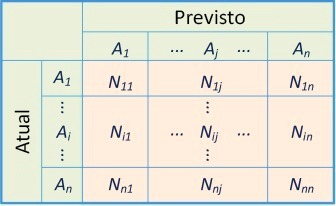
\includegraphics[width=0.6\textwidth]{./dados/figuras/matriz-de-confusao}
    \fonte{Adaptado de \cite{Deng2016}}
    \label{fig:matriz-confusao}
\end{figure}

Uma matriz de confusão é composta por duas dimensões, sendo elas os valores reais e os valores previstos, onde eventualmente eles serão usados para obter uma classificação do método avaliado de acordo com o seu desempenho \cite{Deng2016}. Existe demasiados modelos para se obter os valores da performance do objeto estudado, sendo as medidas mais comuns apresentadas a segui:

\begin{itemize}
   \item Acurácia (AC):
   \begin{description}
    \item Medida usada para calcular o total de previsões corretas dentro dos resultados obtidos
    \begin{equation}
        AC=\sum_{i=1}^nN_{ii}/\sum_{i=1}^n\sum_{j=1}^nN_{ij}
    \label{eq:mc-acuracia}
    \end{equation}
    \end{description}
    \item Precisão (PC):
    \begin{description}
    \item Medida usada para saber a exatidão obtida por determinada classe analisada
    \begin{equation}
        PC_i=N_{ii}/\sum_{k=1}^nN_{ki}
    \label{eq:mc-precisao}
    \end{equation}
    \end{description}
    \item Sensibilidade (SB):
    \begin{description}
    \item Medida usada para saber a probabilidade de acerto de uma determinada classe
    \begin{equation}
        SB_i=N_{ii}/\sum_{k=1}^nN_{ik}
        \label{eq:mc-sensibilidade}
    \end{equation}
    \end{description}
    \item F-Score (Fscore):
    \begin{description}
    \item Medida usada para obter a média harmônica entre a precisão e a sensibilidade
    \begin{equation}
        Fscore_i=\frac{2\times PC_i\times SB_i}{PC_i+SB_i}
        \label{eq:mc-fscore}
    \end{equation}
    \end{description}
\end{itemize}